\chapter{National Competition on DUAL-IPA}

\section{Overview of the Competition}

Bengali Text to IPA (International Phonetic Alphabet) Transcription is an area that has seen relatively limited development compared to other languages, despite Bengali being one of the world's most widely spoken native languages. There is a growing need for automated systems that can accurately convert Bengali text into IPA notation due to the vast audience and various applications in linguistics, language learning, and phonetic research. Having this in mind, we welcome participants to participate in DataVerse, a part of ITVerse 2023 organized by IIT Software Engineers' Community (IITSEC) as we partner with Bengali.AI to advance research in Bengali text to IPA domain.




\section{Competition Schedule}

\textbf{Initial Round:} Was held on Kaggle from October 9th to November 1st. Participants are expected to build and train models during this phase. The top 15 registered teams from this round was invited to join us in the final round.
\\
\textbf{Final Round:} Was held onsite at the Institute of Information Technology, University of Dhaka on 5th November. Only invited teams got a chance to present their work in front of the judge's panel, where they had to submit an IEEE/ACM (2 column) paper. Furthermore, their inference notebooks were evaluated on a hidden dataset.

\newpage

\section{NLP Wrokshop}
A Workshop titled \textbf{Hands-on NLP Workshop: Bengali Transcription Modeling} was arranged in collaboration with Bengali.AI and the organizers where Asif Shahriyar(Coordinator, Bengali.AI) was the host and Dr. Ahmedul Kabir(Associate Professor, IIT, University of Dhaka) was a guest speaker.

 \begin{figure*}[htbp]
    \centering
    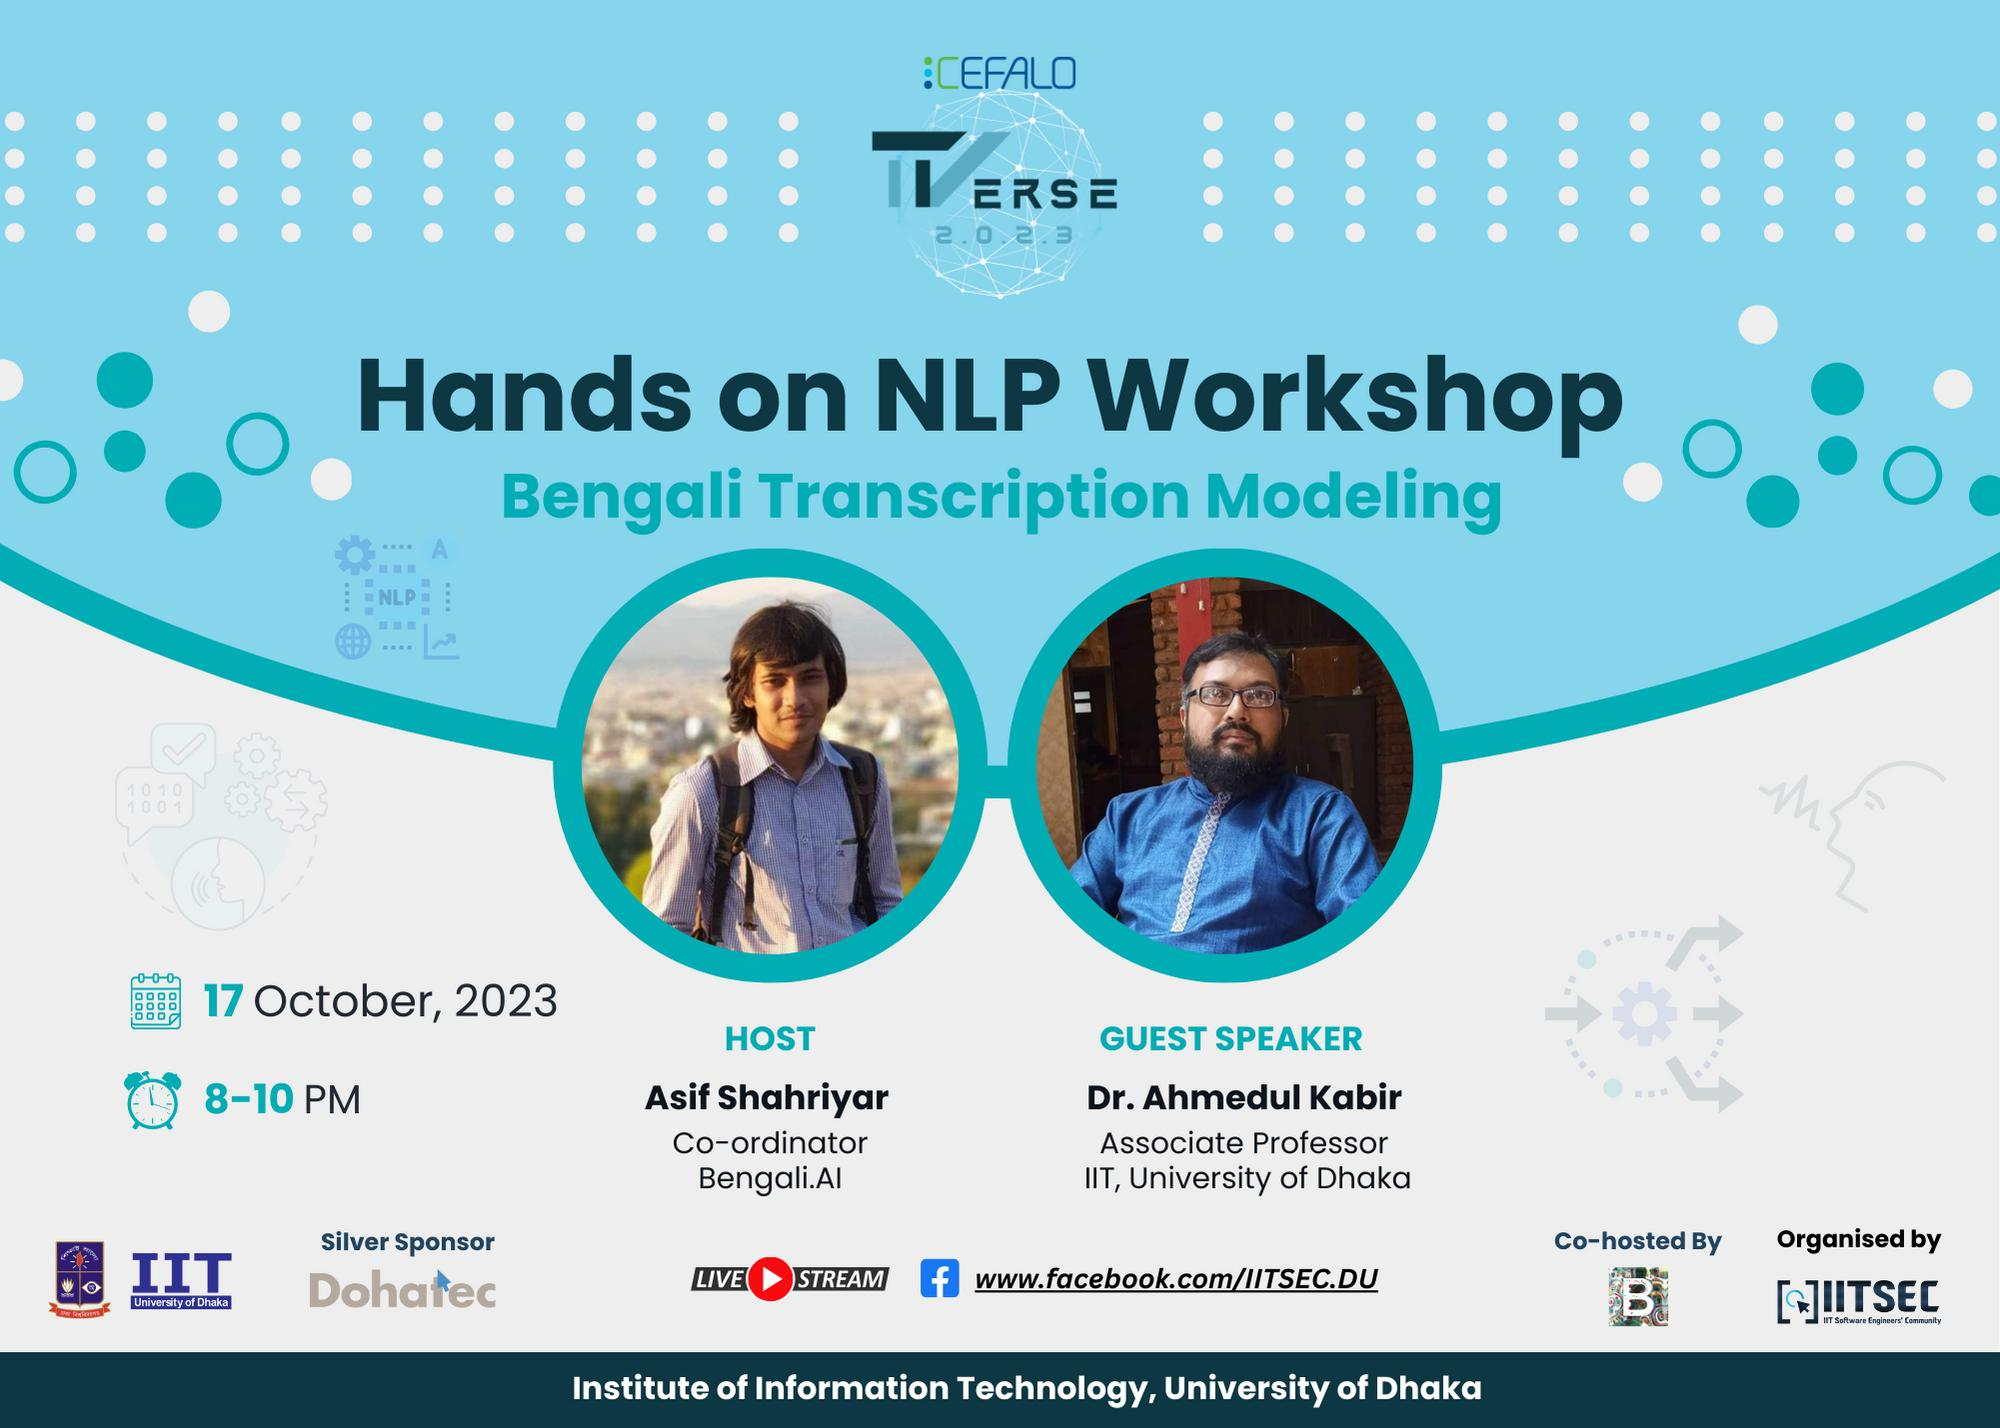
\includegraphics[width=\textwidth]{Images/Screenshot/NLP Workshop.jpg}
    \caption{Hands-on NLP Workshop: Bengali Transcription Modeling}
    \label{fig:workshop}
\end{figure*} 

\section{Scoring}
The scoring weights are divided in the following way - \\
\textbf{Round 1 Public Standing :} 12\% \\
\textbf{Round 1 Private Standing :} 18\% \\
\textbf{Hidden Evaluation :} 50\% \\
\textbf{Paper and Presentation :} 20\% \\

 \begin{figure*}[htbp]
    \centering
    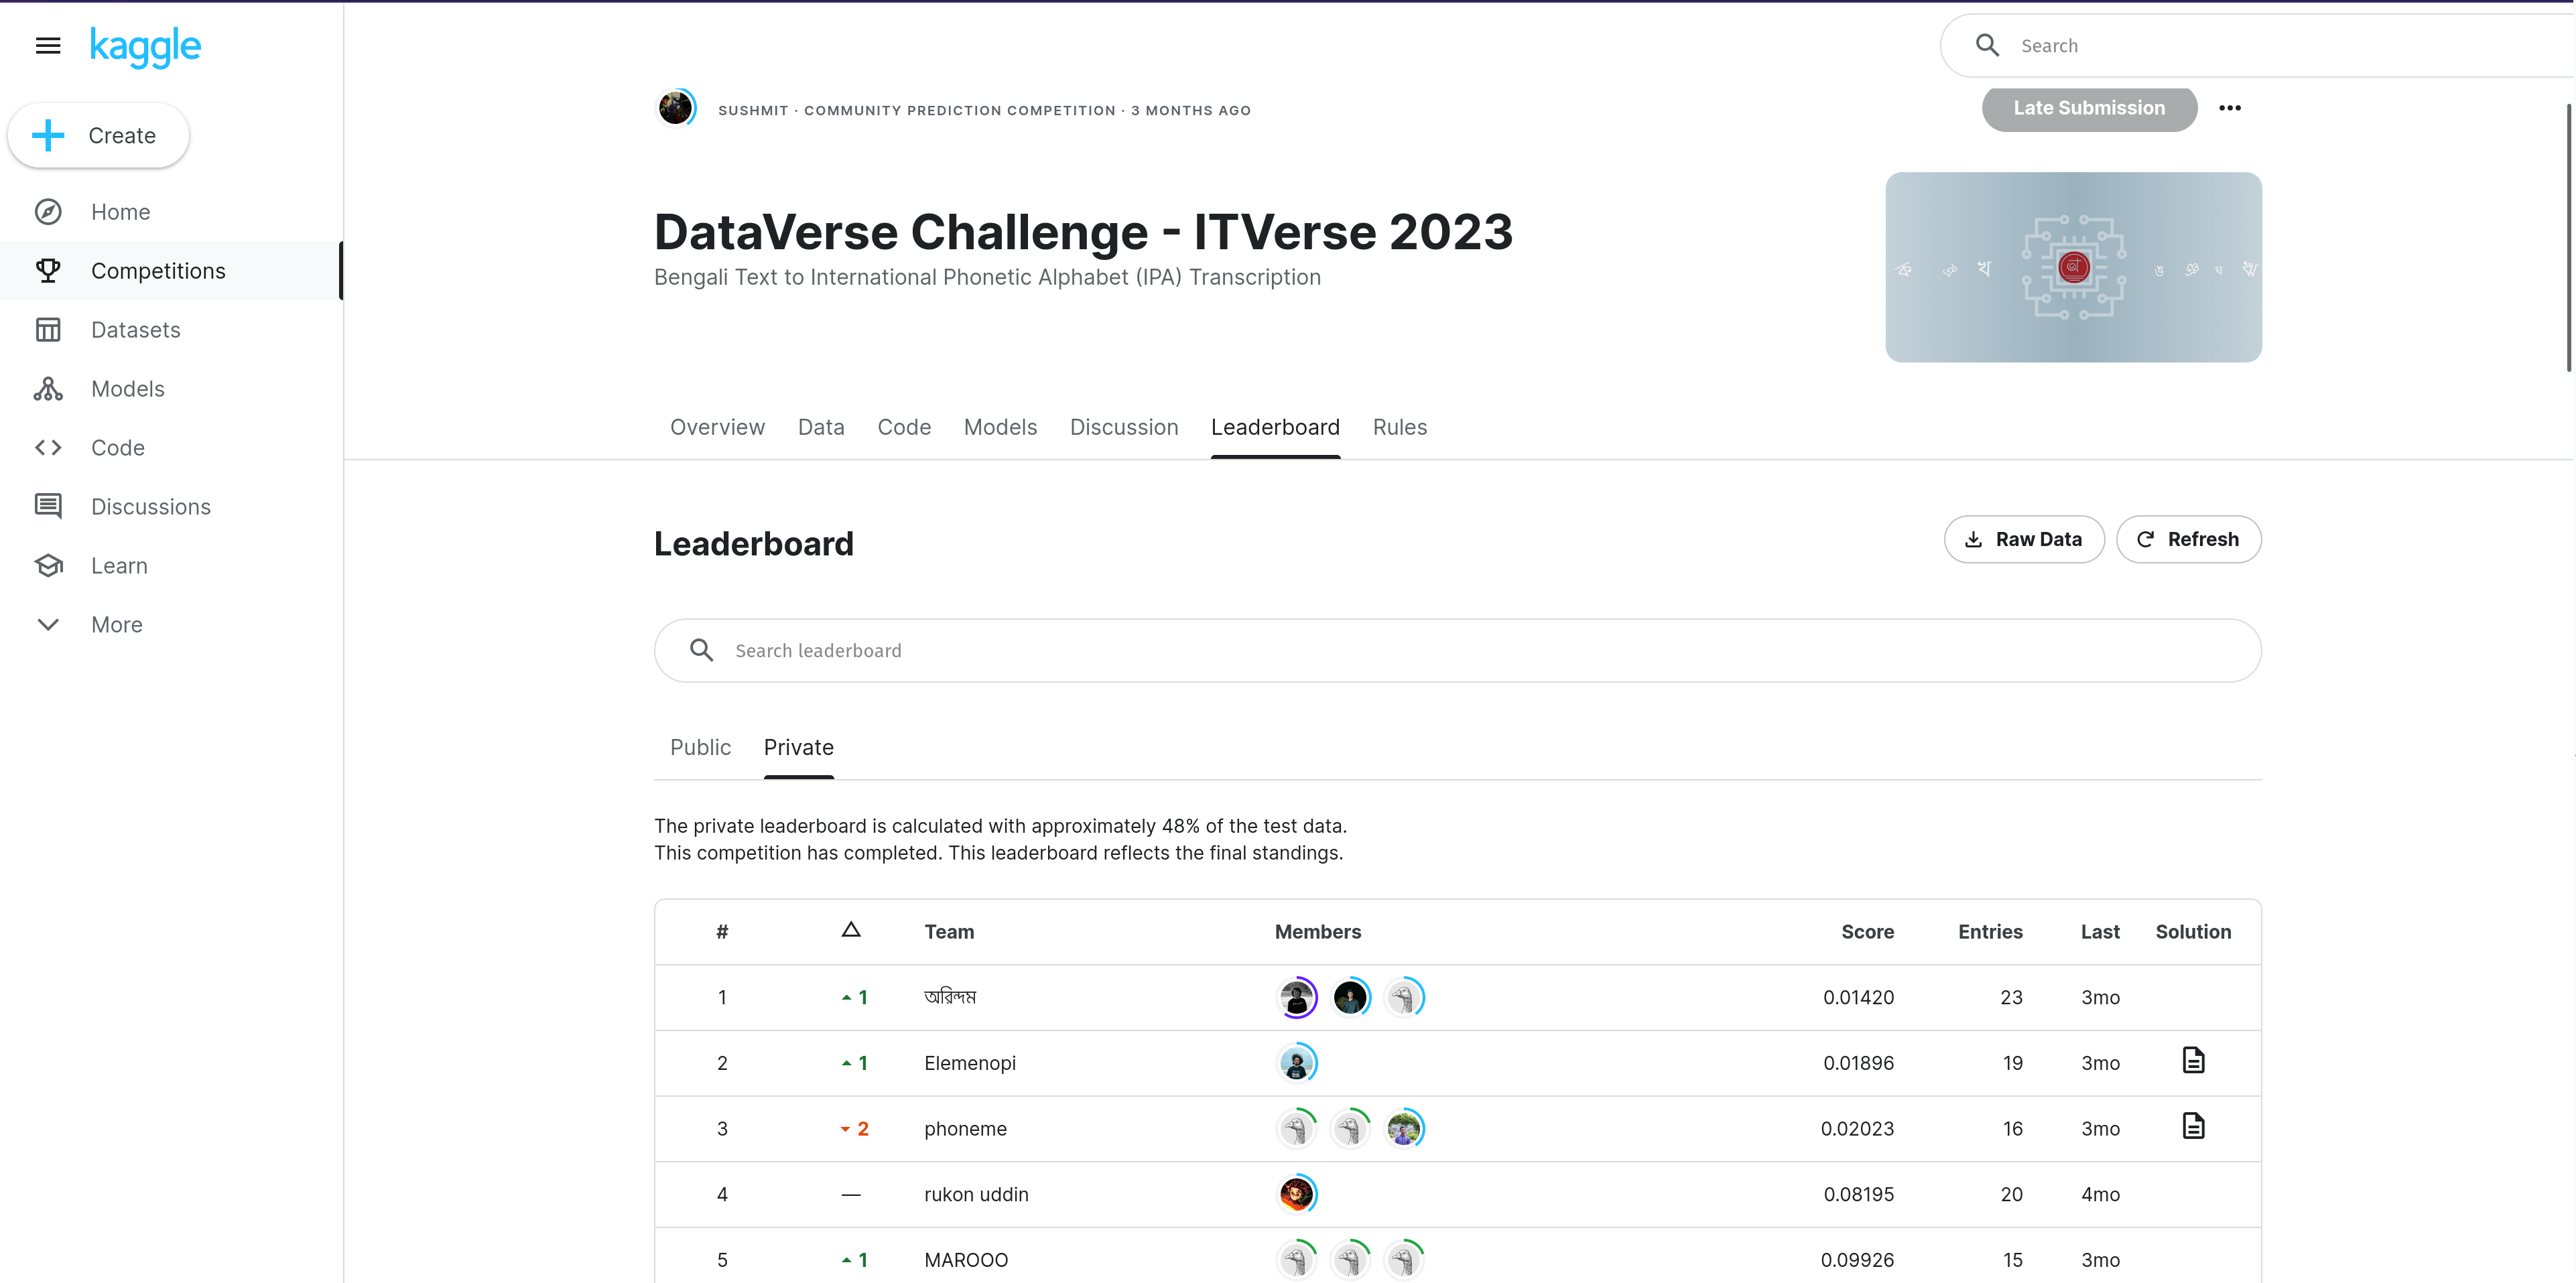
\includegraphics[width=\textwidth]{Images/Screenshot/ITVersre.png}
    \caption{ITVersre 2023, DataVerese segment leaderboard from Kaggle}
    \label{fig:leaderboard}
\end{figure*} 

\section{Goal of the Competition}

The goal of this competition is to recognize model IPA transcription from Bengali texts(Remember the Greek characters in the dictionary, to help us find out the accurate pronunciation of words? That was International Phonetic Alphabet (IPA) transcription! They had to build models trained on a linguist validated dataset containing Bengali text from different domains. The test set contains numbers, loan-words and domain-specific words to add to the challenge.

Their efforts could improve Bengali computational linguistics and NLP research using the first Bengali sentence level IPA transcription dataset from Bengali.AI. In addition, Their submissions have been among the first open-source IPA transcription methods for Bengali.

\newpage
\section{Evaluation}

Submissions were evaluated by a mean Word Error Rate, proceeding as follows:
\begin{itemize}
    \item The WER is computed for each instance in the test set.
    \item The WERs are averaged within domains, weighted by the number of words in the sentence.
    \item The (unweighted) mean of the domain averages is the final score.
\end{itemize}  

\section{Competition Statistics}
\begin{itemize}
    \item \textbf{Total Participants:} 104
    \item \textbf{Teams:} 64
    \item \textbf{Final Model Submission:} 11
\end{itemize}

 \begin{figure*}[htbp]
    \centering
    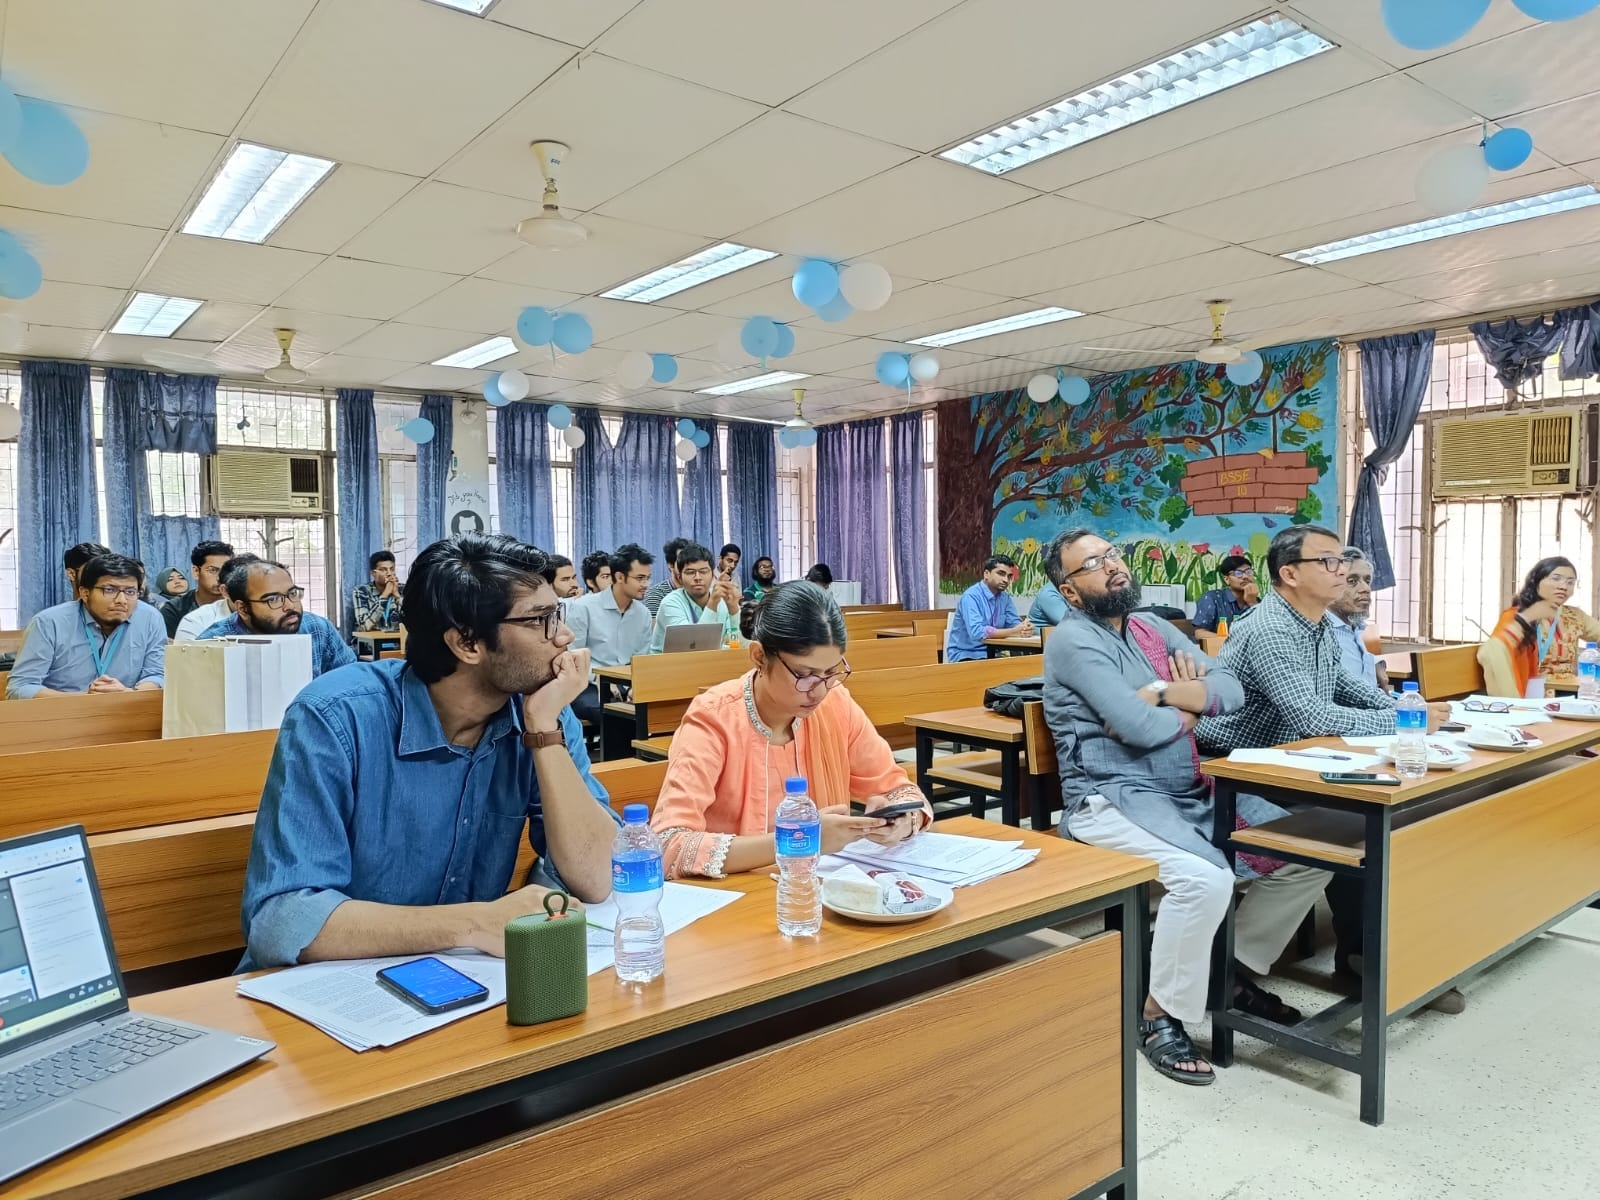
\includegraphics[width=\textwidth]{Images/Screenshot/Dataverse_Judghing.jpg}
    \caption{Glimpse from ITVersre 2023, DataVerese segment}
    \label{fig:glimpse}
\end{figure*} 

 \begin{figure*}[htbp]
    \centering
    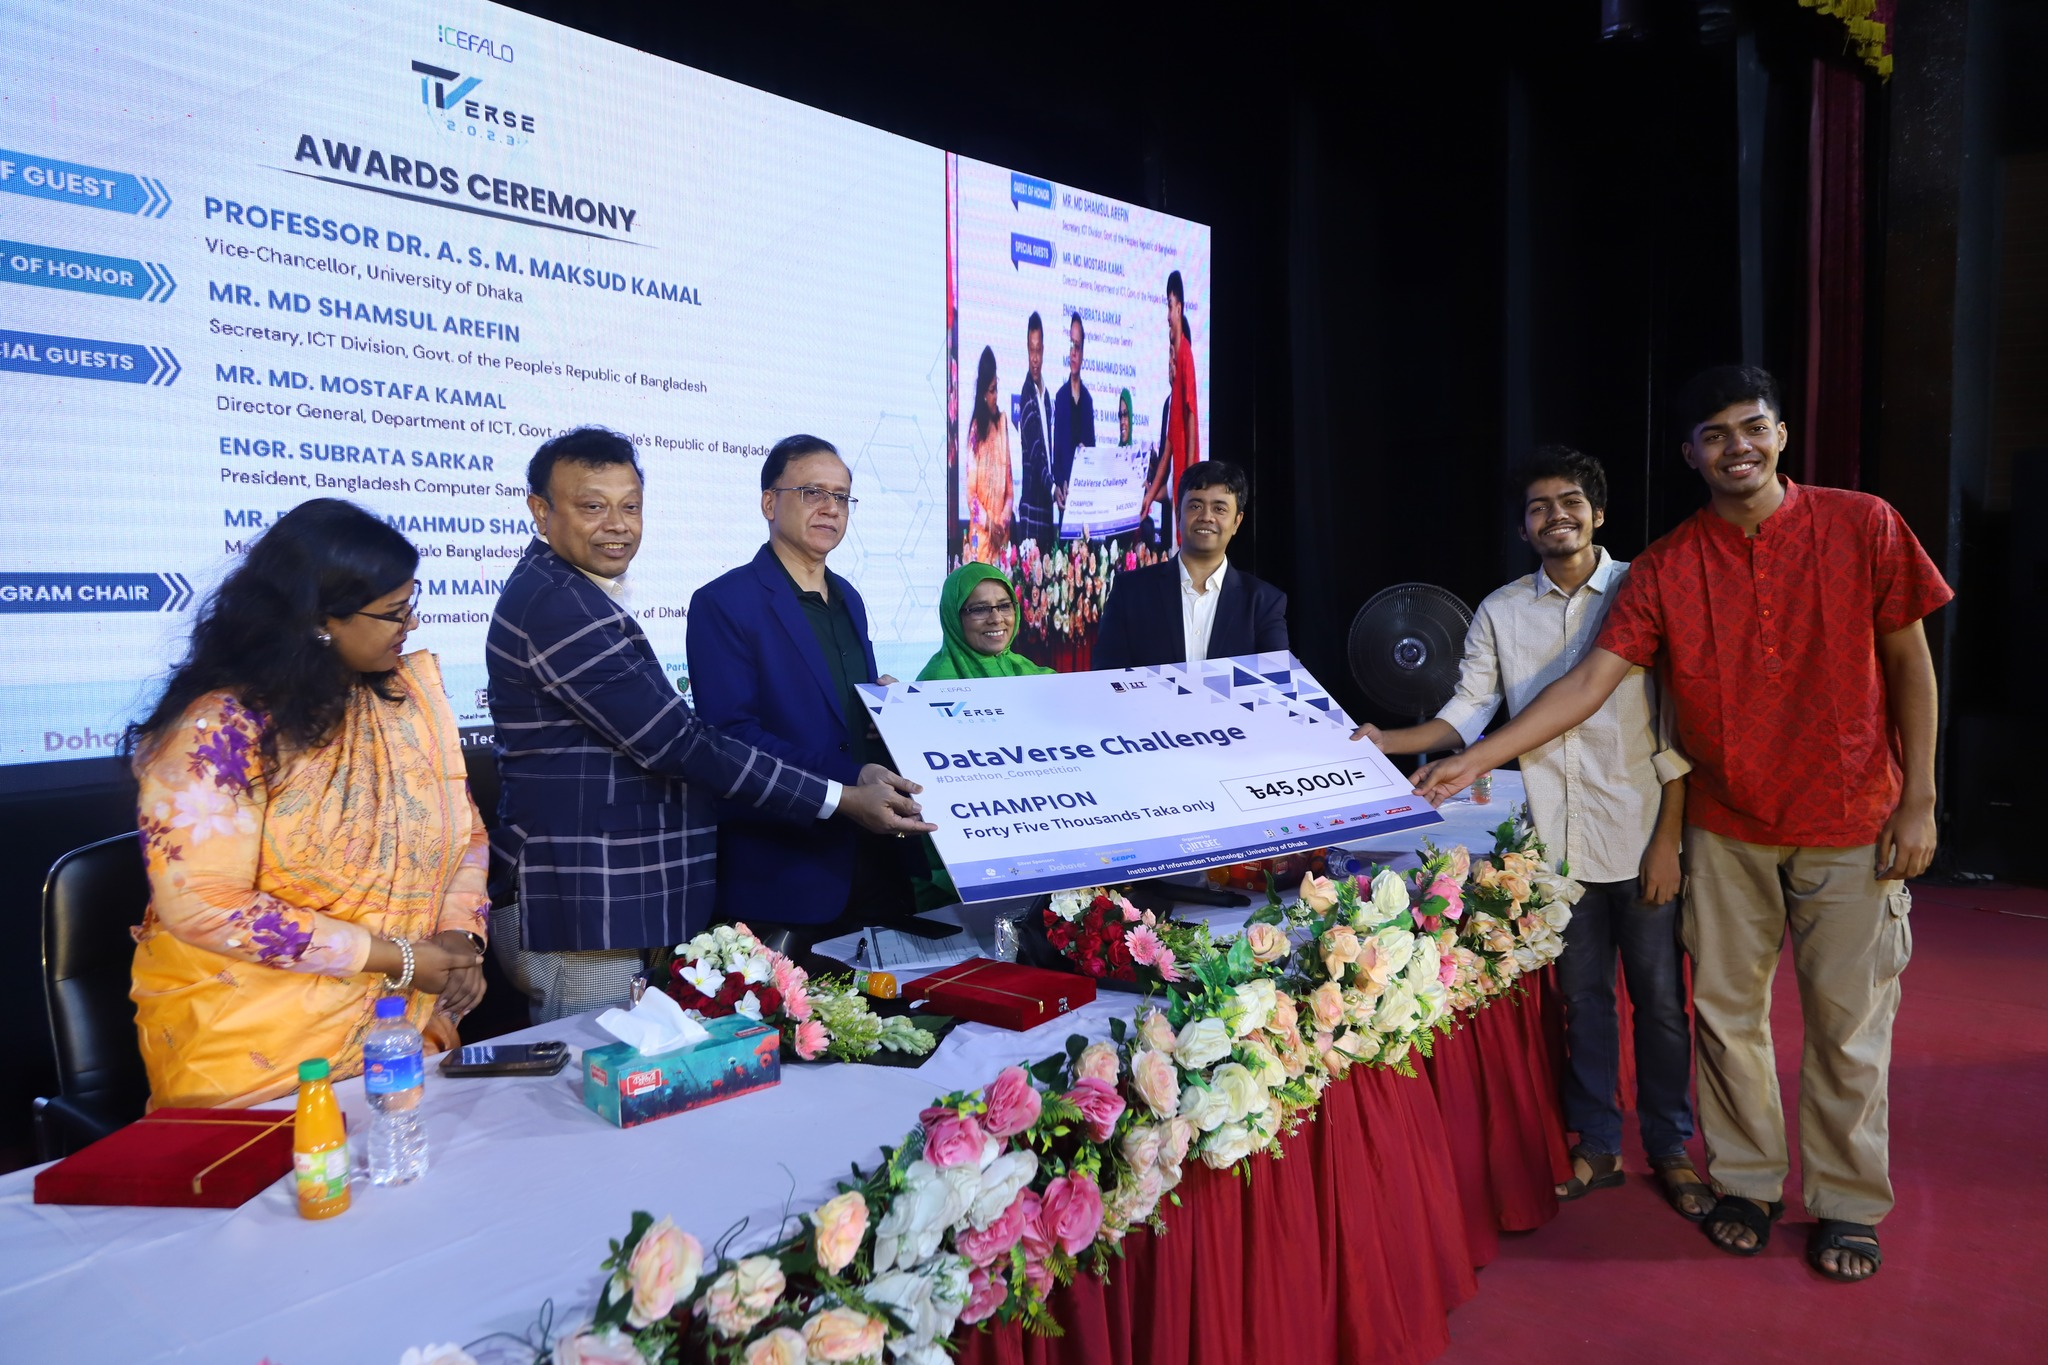
\includegraphics[width=\textwidth]{Images/Screenshot/Dataverse_Champ.jpg}
    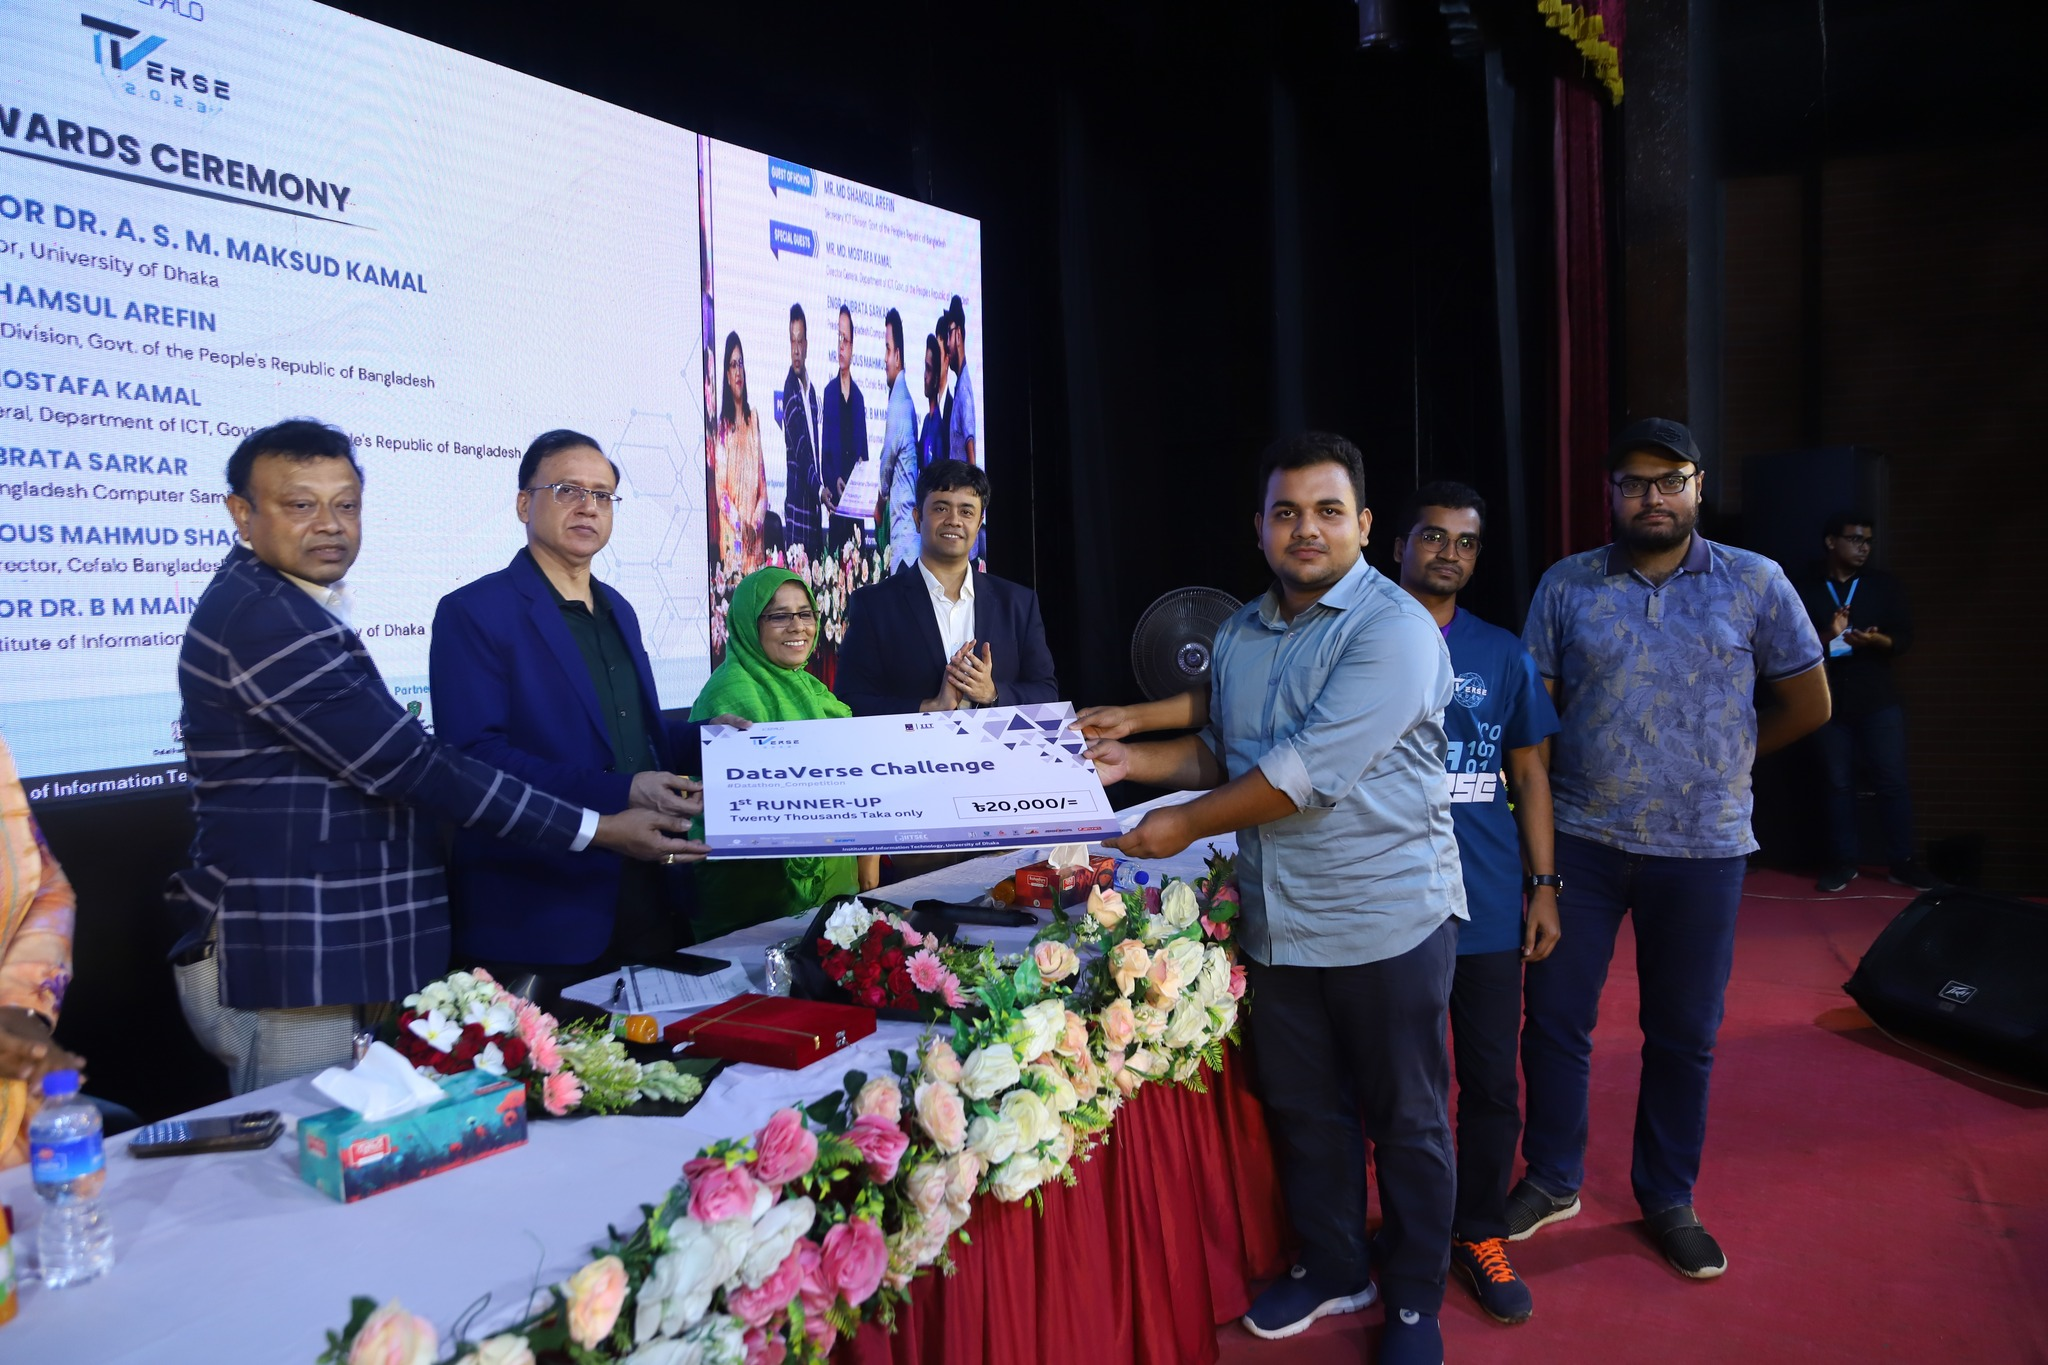
\includegraphics[width=\textwidth]{Images/Screenshot/Dataverse_runner.jpg}
    \caption{Prize Giving Ceremony ITVersre 2023, DataVerese segment}
    \label{fig:prize_giving}
\end{figure*} 
